\documentclass[ignorenonframetext,]{beamer}
\setbeamertemplate{caption}[numbered]
\setbeamertemplate{caption label separator}{: }
\setbeamercolor{caption name}{fg=normal text.fg}
\beamertemplatenavigationsymbolsempty
\usepackage{lmodern}
\usepackage{amssymb,amsmath}
\usepackage{ifxetex,ifluatex}
\usepackage{fixltx2e} % provides \textsubscript
\ifnum 0\ifxetex 1\fi\ifluatex 1\fi=0 % if pdftex
  \usepackage[T1]{fontenc}
  \usepackage[utf8]{inputenc}
\else % if luatex or xelatex
  \ifxetex
    \usepackage{mathspec}
  \else
    \usepackage{fontspec}
  \fi
  \defaultfontfeatures{Ligatures=TeX,Scale=MatchLowercase}
\fi
% use upquote if available, for straight quotes in verbatim environments
\IfFileExists{upquote.sty}{\usepackage{upquote}}{}
% use microtype if available
\IfFileExists{microtype.sty}{%
\usepackage{microtype}
\UseMicrotypeSet[protrusion]{basicmath} % disable protrusion for tt fonts
}{}
\newif\ifbibliography
\hypersetup{
            pdftitle={Analyais on external debt and currency crisis in Emerging markets},
            pdfauthor={Liumin Chen \& Tingjie Meng},
            pdfborder={0 0 0},
            breaklinks=true}
\urlstyle{same}  % don't use monospace font for urls

% Prevent slide breaks in the middle of a paragraph:
\widowpenalties 1 10000
\raggedbottom

\AtBeginPart{
  \let\insertpartnumber\relax
  \let\partname\relax
  \frame{\partpage}
}
\AtBeginSection{
  \ifbibliography
  \else
    \let\insertsectionnumber\relax
    \let\sectionname\relax
    \frame{\sectionpage}
  \fi
}
\AtBeginSubsection{
  \let\insertsubsectionnumber\relax
  \let\subsectionname\relax
  \frame{\subsectionpage}
}

\setlength{\parindent}{0pt}
\setlength{\parskip}{6pt plus 2pt minus 1pt}
\setlength{\emergencystretch}{3em}  % prevent overfull lines
\providecommand{\tightlist}{%
  \setlength{\itemsep}{0pt}\setlength{\parskip}{0pt}}
\setcounter{secnumdepth}{0}

\title{Analyais on external debt and currency crisis in Emerging markets}
\author{Liumin Chen \& Tingjie Meng}
\date{April.29 2019}

\begin{document}
\frame{\titlepage}

\begin{frame}{Problem statement and Background}

Frequent currency crisis in EMEs: Why so vulnerable?

\begin{itemize}
\tightlist
\item
  a high level of external debt
\item
  external shocks
\item
  politicial instability
\item
  GDP level
\end{itemize}

\end{frame}

\begin{frame}{Problem statement and Background}

\begin{itemize}
\tightlist
\item
  What factors strengthen or weaken the link between external debt and
  currency crisis in EMEs?
\item
  How to predict the possibility of a currency crisis happening in the
  future?
\item
  Policy guidance for central bank policymakers in emerging markets
\end{itemize}

Testable hypothesis:

\begin{itemize}
\tightlist
\item
  EMEs with high external debt are more prone to currency crisis risks
\end{itemize}

\end{frame}

\begin{frame}{Approach}

Variables:

\begin{itemize}
\tightlist
\item
  Dependent variable: possibility of currency crisis (a nominal
  depreciation of 15\% within a year)
\item
  Independent variable: external debt/GNI
\item
  Control variable: GDP per capita, level of democracy, US 3-month
  treasury yield, foreign reserves/total external debt
\end{itemize}

Data access:

\begin{itemize}
\tightlist
\item
  the World Bank Open Data
\item
  the International Monetary Fund (IMF) Open Data
\item
  the Polity IV Project conducted by the Center for Systemic Peace
\end{itemize}

\end{frame}

\begin{frame}{Methods}

Data visualizations

\begin{itemize}
\tightlist
\item
  The connection between currency crisis and external debt
\item
  The connection between currency crisis and control variables
\end{itemize}

Logit model

\begin{itemize}
\tightlist
\item
  Model the probability of a currency crisis happening given all
  variables
\item
  (external debt/GNI; GDP per capita, level of democracy, US 3-month
  treasury yield, foreign reserves/total external debt)
\end{itemize}

Machine learning

\begin{itemize}
\tightlist
\item
  Predict the classification
\item
  Several models (K nearest neighbours, CART, and Random Forest)
\end{itemize}

\end{frame}

\begin{frame}{Result: data visualizations}

\begin{center}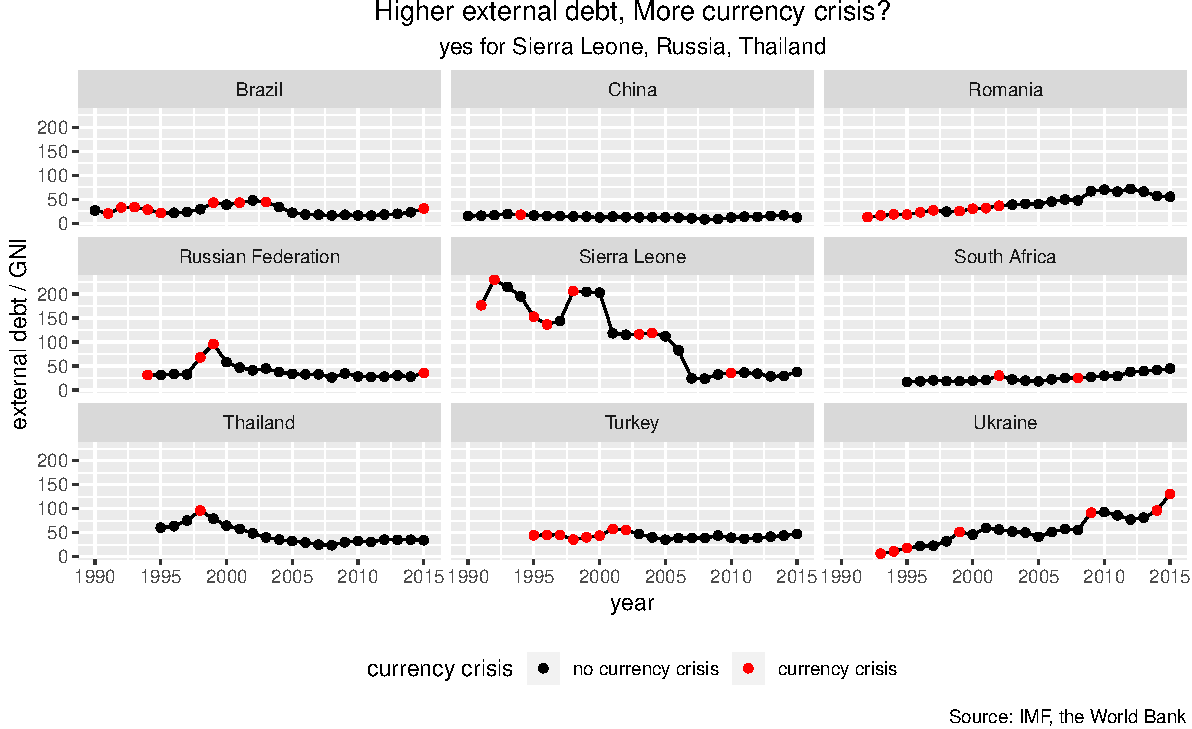
\includegraphics{beamer-pre_files/figure-beamer/unnamed-chunk-5-1} \end{center}

\end{frame}

\begin{frame}

\begin{center}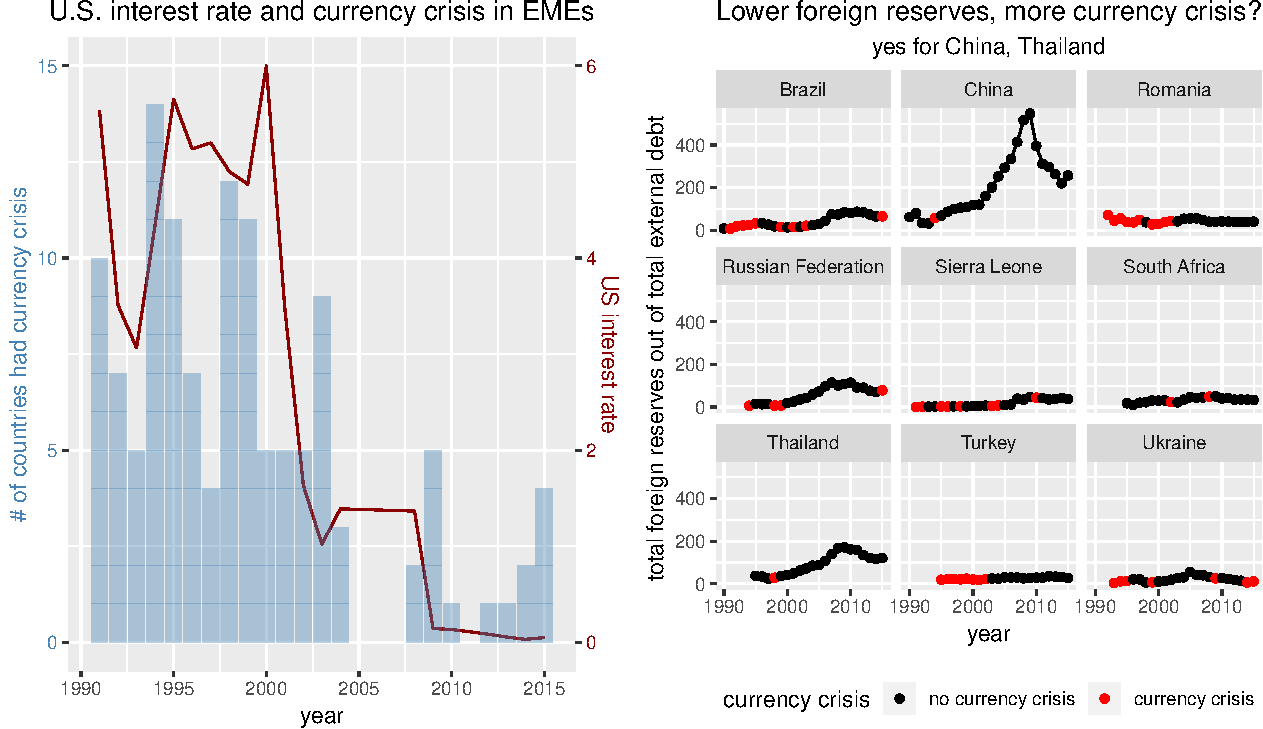
\includegraphics{beamer-pre_files/figure-beamer/unnamed-chunk-9-1} \end{center}

\end{frame}

\begin{frame}{Result: Logit model}

a positive correlation between independent variable of interest and the
dependent variable, statistically significant at the 0.1\% level.

This supports our main hypothesis that countries who have borrowed
excessively in foreign currency are more prone to currency crisis risks.

a negative correlation between the ratio of foreign reserves to a
country's total external debt in the previous year and the dependent
variable

also a negative correlation between GDP per capita in the previous year
and the probability of a currency crisis happening

\end{frame}

\begin{frame}

\begin{center}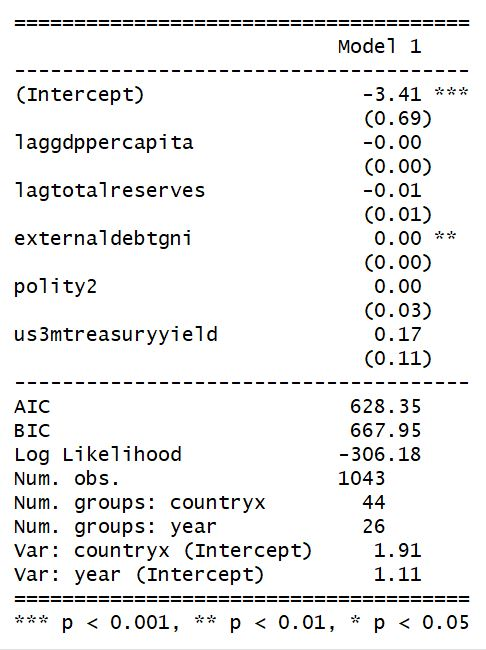
\includegraphics{C:/Users/Meng/Desktop/Spring2019/DataScience/group project/new project/New-Group-Project/graphs/logit} \end{center}

\end{frame}

\begin{frame}

\begin{center}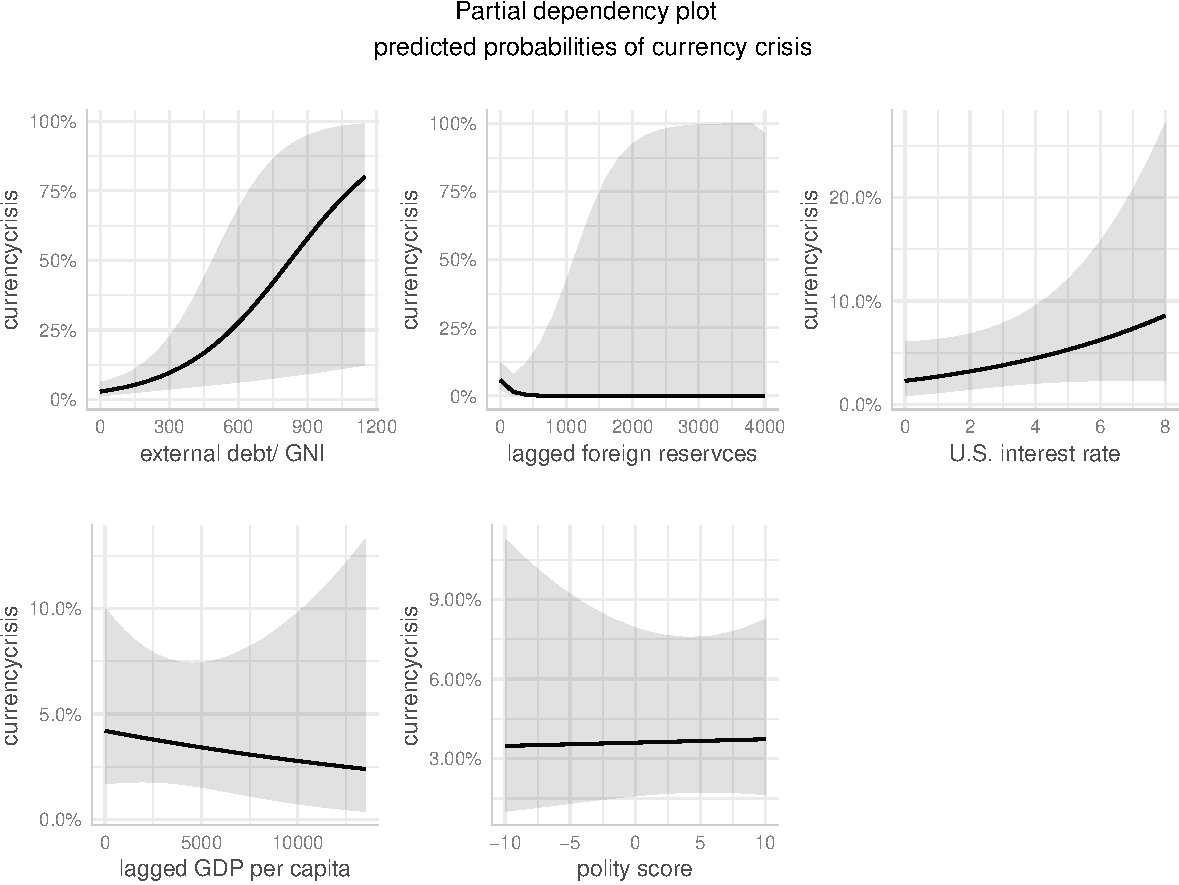
\includegraphics{beamer-pre_files/figure-beamer/unnamed-chunk-26-1} \end{center}

\end{frame}

\begin{frame}{Result: Machine learning}

\begin{center}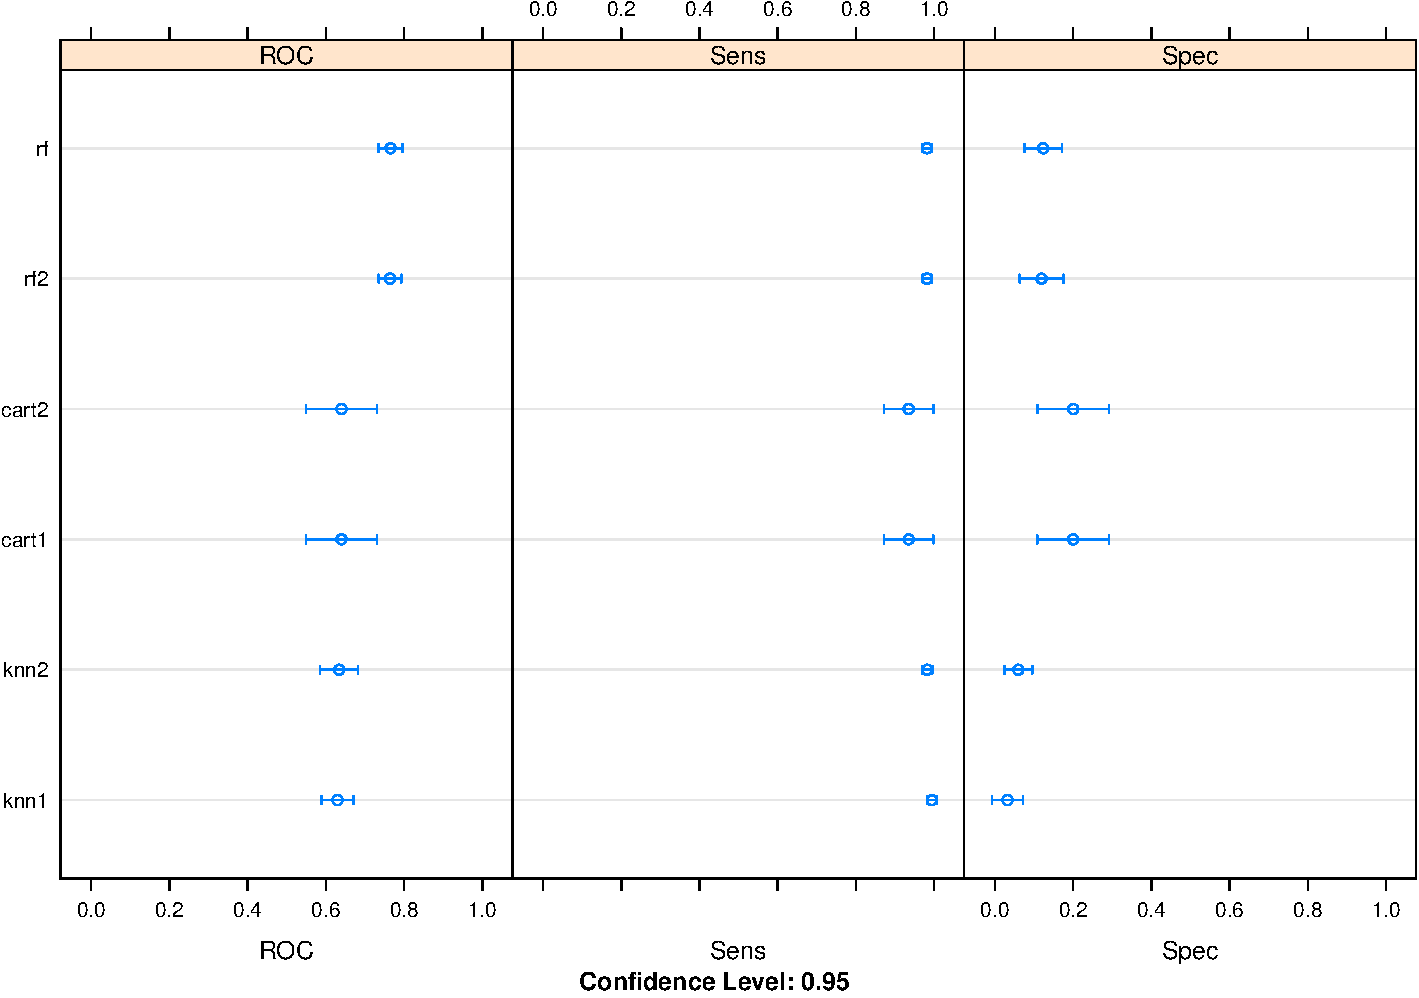
\includegraphics{beamer-pre_files/figure-beamer/unnamed-chunk-54-1} \end{center}

\end{frame}

\begin{frame}{Predictive performance for mod2\_rf}

\begin{center}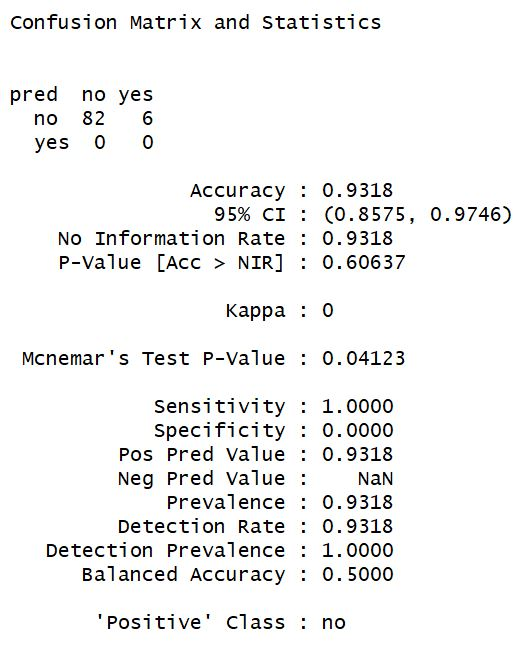
\includegraphics{C:/Users/Meng/Desktop/Spring2019/DataScience/group project/new project/New-Group-Project/graphs/confusion matrix} \end{center}

\end{frame}

\begin{frame}{Most important variables}

\begin{center}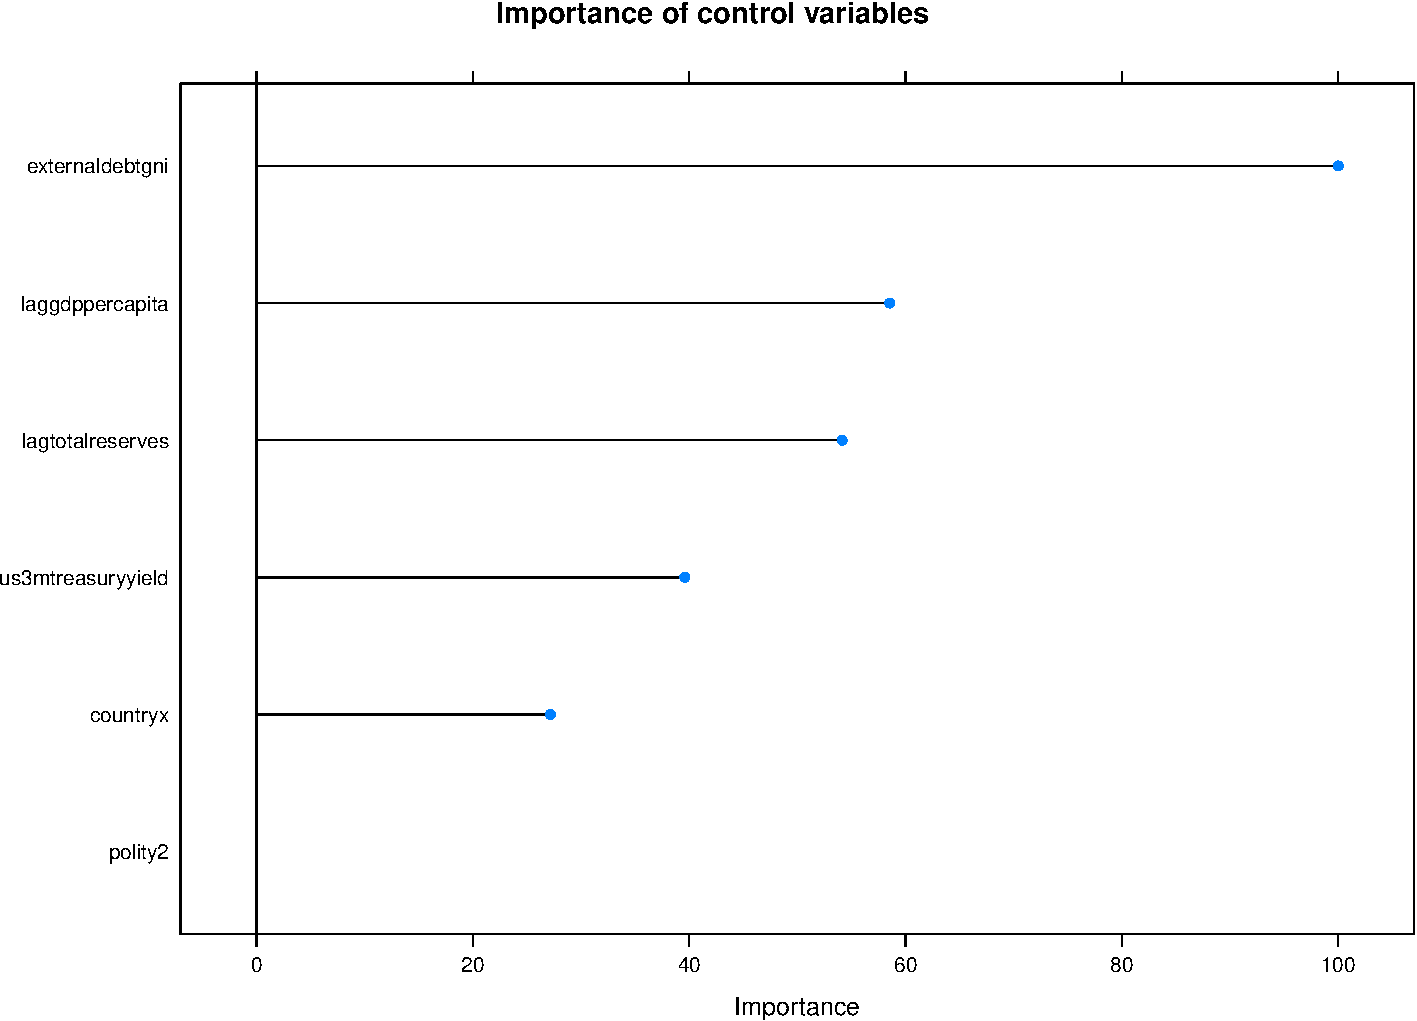
\includegraphics{beamer-pre_files/figure-beamer/unnamed-chunk-57-1} \end{center}

\end{frame}

\begin{frame}{Lessons learned}

\begin{itemize}
\tightlist
\item
  EMEs should control external debt level
\item
  Stock foreign reserves
\item
  Boost GDP
\item
  Monitor U.S. interest rate volatility
\end{itemize}

\end{frame}

\begin{frame}{Next steps}

\begin{itemize}
\tightlist
\item
  Find a better proxy for political instability
\item
  More variables to include: economic structure \& exchange rate regime
\item
  Expand the time rage
\end{itemize}

\end{frame}

\end{document}
